\documentclass{article}

\usepackage{subfig}
\usepackage{float}
\usepackage{graphicx}
\usepackage{algorithm}
\usepackage{algpseudocode}
\usepackage{changepage}
\usepackage{amsmath}
\usepackage[driver=pdftex]{geometry}
\DeclareMathOperator*{\argmax}{argmax}
\DeclareMathOperator*{\argmin}{argmin}




\begin{document}
\begin{titlepage}
	
	
	\begin{center}
		\vspace{2 cm}
		{\Large \textsc{Simone Quadrelli} }
	\end{center}
	
	
	\begin{figure}[H]
		\vspace{2 cm}
		\centering
		
\includegraphics[width=0.30\linewidth]{tesiSCIENZE_TECNOLOGIE.jpg}
		
	\end{figure}
	
	\begin{center}
		\vspace{2 cm}
		{\Large \textsc{Genetic algorithm Monte Carlo} }
	\end{center}

	\par
	\vspace{3 cm}
	
	\begin{center}
		{\large Academic year 2019 - 2020}
	\end{center}
\end{titlepage}

\pagenumbering{gobble}
\newpage 
\pagenumbering{roman}
\tableofcontents
\listoftables
\listoffigures
\newpage

\pagenumbering{arabic}

\section*{Abstract}
The aim of this project is to solve the travelling salesman problem (TSP) which consists in finding the shortest cycle among all the cities. The problem is a \textit{NP-hard} problem and therefore there exist no feasible algorithm to solve if for any possible set of cities in input. The appromximately optimal solution was computed by the simulated annealing, while the possible cycles are produced by a genetic algorithm.

\section{Introduction}
The travelling salesman problem consists in finding the shortest route a travelling salesman has to take to visit all the city he must reach only once and to return to the starting point. The route described is called in graph theory \textit{hamiltonian cycle} (i.e a cycle that pass through each vertex of a graph just once), indeed the oldest and more technical formulation of the problem was proposed by Hamilton. \\
An algorithm that provides a solution to TSP can be exploited in a wide variety of applications: indeed it can be used in logistics to optimize the path of vehicles and therefore to reduce costs.
It is possible to model the problem usign an undirected, weighted and fully connected graph \footnote{For an hamiltinian cycle to exist the graph must be at least connected} $G = (N,E)$, where $N$ is the set of the cities to visit and $E =  N \times N$ is the weight of the path. In this particular instance of the probelm the weights correspond to the euclidean between each couple of cities.
THe mailtonian cycle can be defined as a sequence $(n_0, .., n_{k-1})$ of length k such that $n_i \neq n_j \; \forall i,j \in \{1,..., |N|\}$ and such that $(i,j) \in E \; \forall i,j \in \{1,..., |N|\}$
The most naive solution is to compute all the possible paths but they are factorial in the number of cities $n$ in input. The number of possible cycles is $(n-1)!$ and grows faster that $2^n$ (i.e $2^n = o(n!)$). Therefore even if it was possible to find them in constant time the algorithm will have an expnential time complexity and would not be solved in finite time for large $n$. 
More techically, TSP is an NP-hard problem. A NP-hard problem is a problem at least as hard as the hardest NP-complete problem. NP-complete problem is a problem that can be solved in polynomial time by a non-deterministic algorithm. For such a class of problem there exists no polynomial algorithm that can solve the problems and may not exist, still noone was able to prove that such algorithms does not exists.
\begin{figure}
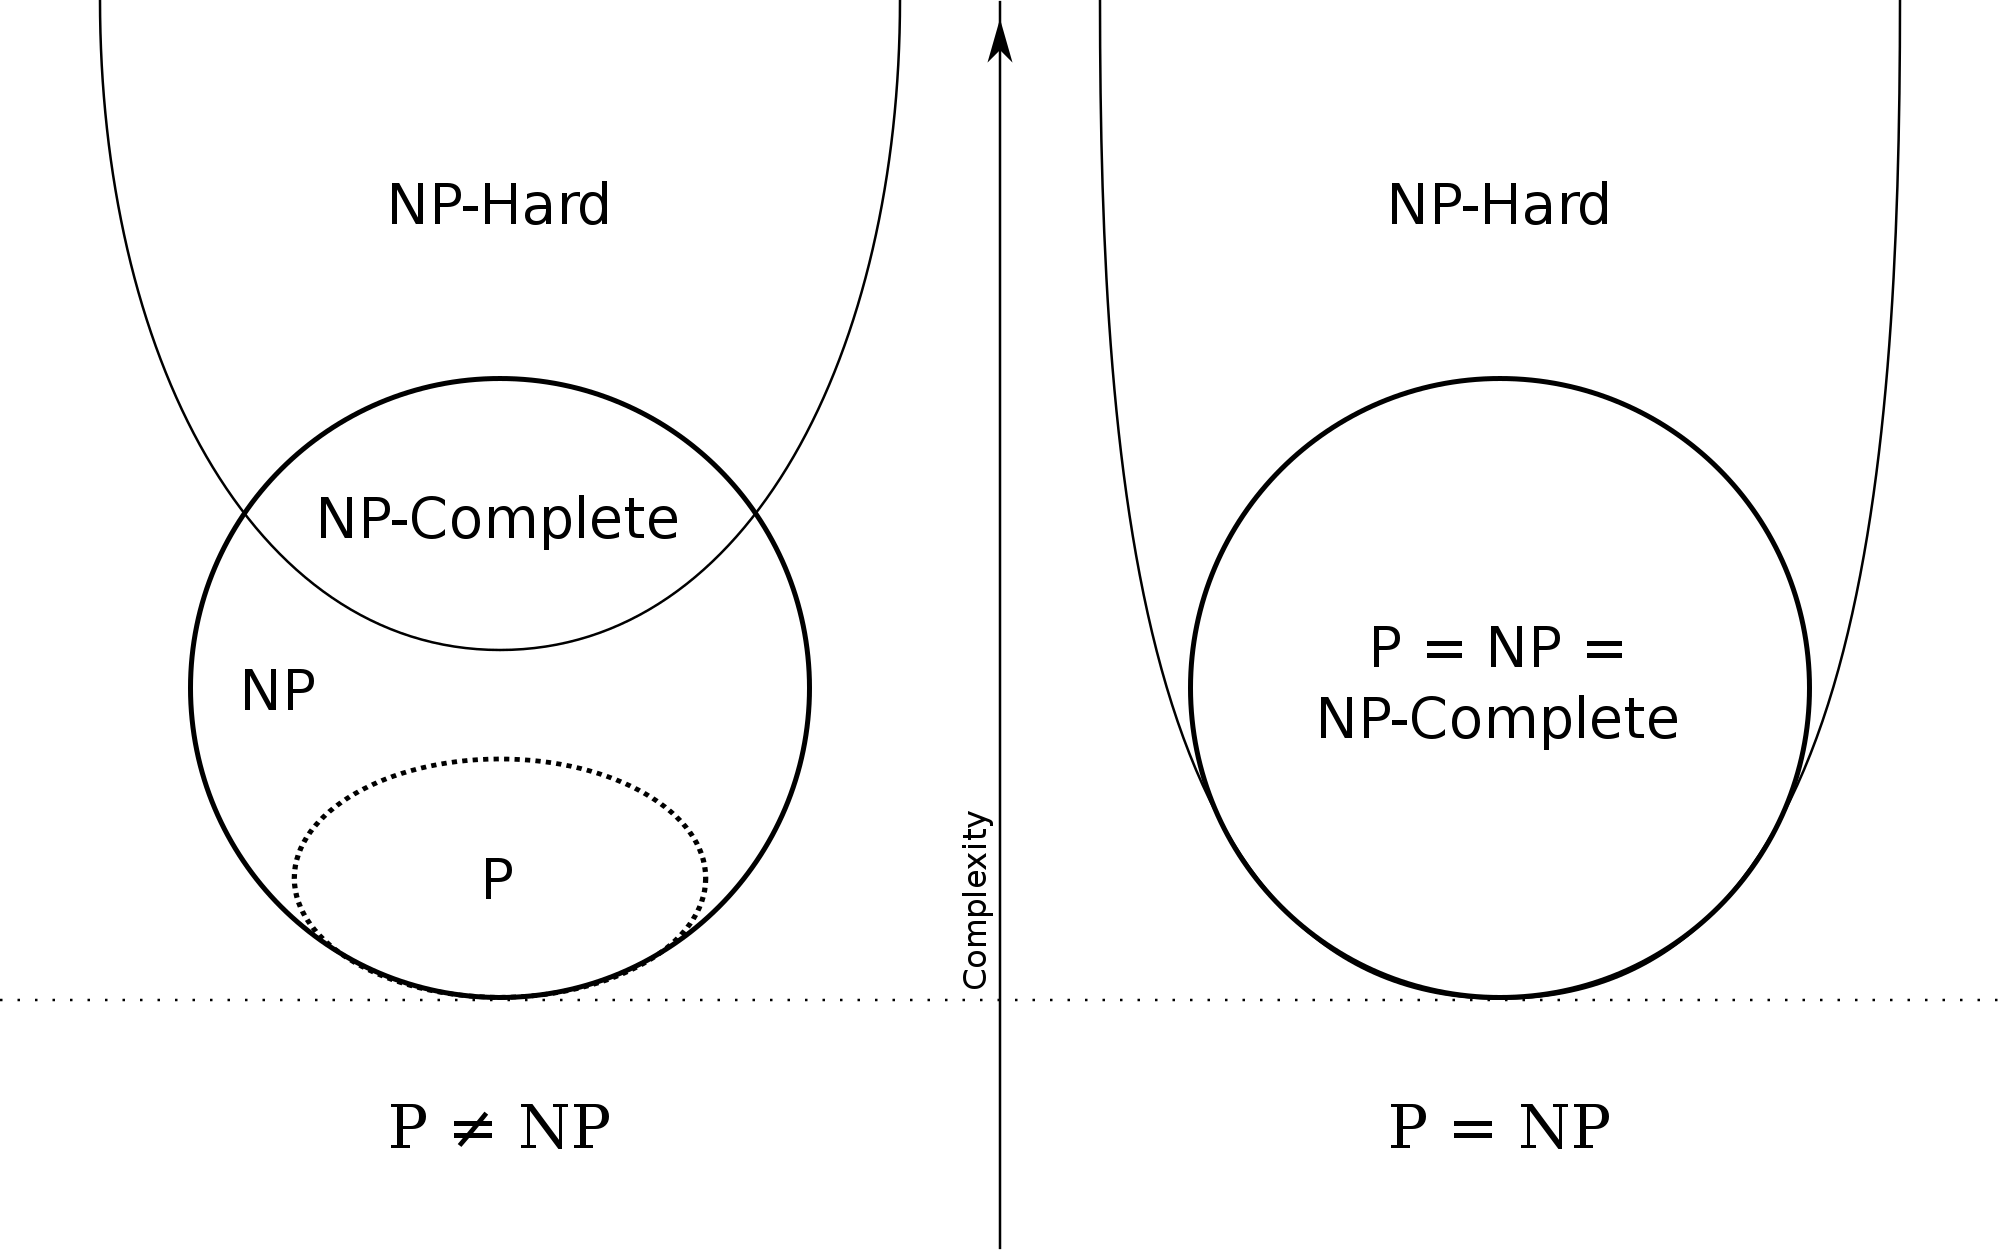
\includegraphics[scale=1]{complexity_classes.png} 
\centering
\end{figure}
Bearing in mind the complexity problem to face, the most reasonable solution is to solve the problem approximately. The technique I to generate the possible hamiltonian cycles is a genetic algorithm, while the choice of the fittest hamiltonian cycle is done by the simulated annealing algorithm

\section{Simulated annealing}
Simulated annealing (SA) is a technique that mimic the behaviour of heated materials in metallurgy that can be slowly cooled down, this process decreases the impurity and increases the size of the crystals. It is a technique that pproximates the global optimal solution when the solutions is to be searched in an enormous space. SA is a metaheuristic meaning that it is not a probelm specific heuristic and that can be used to reduce the search space of an algorithm, the genetic algorithm in our case.\\
SA very usefull since it does not require any prior information, indeed it just supposes that the states (hamiltonian cycles in our case) are distributed accordingly to the Bolzmann distribution:
\begin{equation}
\exp^{- \beta (cost(new state) - cost(old state))}
\end{equation}
The temperature $T$ stated before is $T = \frac{1}{\beta}$, therefore we start with low values of betas (high temperature) and as the simulation proceeds we increase the values of $\beta$, thus mimicing the decrease in temperature.
The only other information needed is the cost function. For this specific application the cost function is the euclidean distance between the cities. The $(x,y)$ are expressed in latitude and longitude (CONTROLLA L'ORDINE). Therefore given the coordinates of two cities  $(x_1,y_1)$ and $(x_3,y_2)$
\begin{equation}
cost((x_1,y_1),(x_2,y_2)) = \sqrt{(x_1-x_2)^2 + (y_1-y_2)^2}
\end{equation}

\begin{algorithm}[h]
    \begin{algorithmic}[1]
      \Function{simulated annealing}{}
        \State s $\leftarrow$ generate starting state
         \For {b in \textbf{betas}}
         	\For{n in 1,.., number of simulations}
         	\State ns  $\leftarrow$ sample new states with metropolis algorithm
         	\EndFor
        \EndFor
        \State return ns
       \EndFunction
\end{algorithmic}
\end{algorithm}

\section{Metropolis algorithm}

\section{Genetic Algotirthm}
Genetic algorithms are a widespread class of algotirhms that mimic nature. Indeed there are three fundamental operations they perform, each operation is inspired by the theory of evolution by Darwin. Among a specie evolution selects the fittest individuals and therefore the algorithm will chose the fittest (i.e shortest) hamiltonian cycles. The breeding of the fittest individuals produces new individuals that inherits traits from the parents, therefore in the crossbreeding phase we mix some subsection of the fittest hamiltonian cycles.
As random mutations can occur in nature but they are not so likely to accur, the algorithms swaps two nodes (cities) with a fixed and low probability.
My own implementation of the algorithms performs the selection operation as follows:
\begin{algorithm}[h]
    \begin{algorithmic}[1]
      \Function{selection}{\textbf{population},n\_paths}
        \State $n\_parents \leftarrow$ unif[2,n\_paths/2]
        \State order the population by fitness
        \State \textbf{fittest\_subpopulation} $\leftarrow$ extract $n\_parents$ in order from the sorted population
        \State return \textbf{fittest\_subpopulation}
       \EndFunction
\end{algorithmic}
\end{algorithm}
\noindent where \textbf{population} is an array of hamiltonian cycles

\begin{algorithm}
    \begin{algorithmic}[1]
      \Function{crossbreeding}{\textbf{fittest\_subpopulation}}
      	\For {i in 1, ..., n\_paths}
  			\State choose parent1 uniformely among the \textbf{fittest\_subpopulation}
  			\State Choose parent2 uniformely among the \textbf{fittest\_subpopulation}
  			\If {parent1 different from parent2}
  				\State choose position1 randomly among unif([0,length of cycles-1)
  				\State choose position2 randomly among unif([0,length of cycles-1)
  				\State divide parent1 in three sections: 
  				\State[parent10:position1] 
  				\State parent1[position1:position2]
  				\State parent1[posotion2:]
  				\State divide parent2 in three sections:
  				\State parent2[0:position1] 
  				\State parent2[position1:position2]
  				\State parent2[posotion2:]
  				\State breed child1 justapposing in the order:
  				\State parent1[0:position1]
  				\State all the cities not in  parent1[0:position1] and not in parent2[posotion2:]
  				\State parent2[posotion2:]
  				\State breed child2 justapposing in the order:
  				\State parent2[0:position1]
  				\State all the cities not in  parent2[0:position1] and not in parent1[posotion2:]
  				\State parent1[posotion2:]
  			\Else
  				\State child1 $\leftarrow$ parent1
  				\State child2 $\leftarrow$ parent1
  			\EndIf
      	\EndFor
        \State \textbf{new\_population} is a vector of the children 
       \EndFunction
\end{algorithmic}
\end{algorithm}
2) Crossbreeding --> obtain new hamiltonian cycles exchanging the gines of the parents
3) Mutation --> exchange genes randomly
\begin{algorithm}[h]
    \begin{algorithmic}[1]
      \Function{mutate}{\textbf{new\_population}, p}
        \State test $\leftarrow$ unif[0,1]
        \If {test $<$ p}
        	\State choose position1 randomly among unif([0,length of cycles-1)
  			\State choose position2 randomly among unif([0,length of cycles-1)
  			\State swap the cities in position1 and position2
        \EndIf
        \State order the population by fitness
        \State \textbf{fittest\_subpopulation} $\leftarrow$ extract $n\_parents$ in order from the sorted population
        \State return \textbf{fittest\_subpopulation}
       \EndFunction
\end{algorithmic}
\end{algorithm}


\begin{algorithm}[h]
    \begin{algorithmic}[1]
      \Function{evolve}{\textbf{population}}
        \State \textbf{fittest\_population} $\leftarrow$ SELECT(\textbf{population})
        \State \textbf{new\_population} $\leftarrow$ CROSSBREED(\textbf{fittest\_population})
       \State \textbf{population} $\leftarrow$ MUTATE(\textbf{new\_population})
       \EndFunction
\end{algorithmic}
\end{algorithm}
\section{dataset}

\section{results}

\end{document}